\chapter{Vibration Pattern Analysis for Haptic Belts}
\label{chapter:vibration_pattern_analysis_for_haptic_belts}

In this Chapter, we provide the user study for vibration patterns to be used on the Tactile Belt described in Chapter \ref{chapter:person_guidance}.


\section{Tactile Belt}
\label{sec:belt}

The belt is made of elastic material so that the vibration motors make contact with the human body and the angle between motors is fixed. This property allows us to represent the 8 cardinal directions consistently for every user.

Upon receiving a vibration pattern, the controller on the belt applies corresponding sequences of voltages to the vibration motors. A vibration pattern incorporate the activation frequency, duration and rhythm of vibrations for all motors.

\begin{figure}[ht!]
\centering
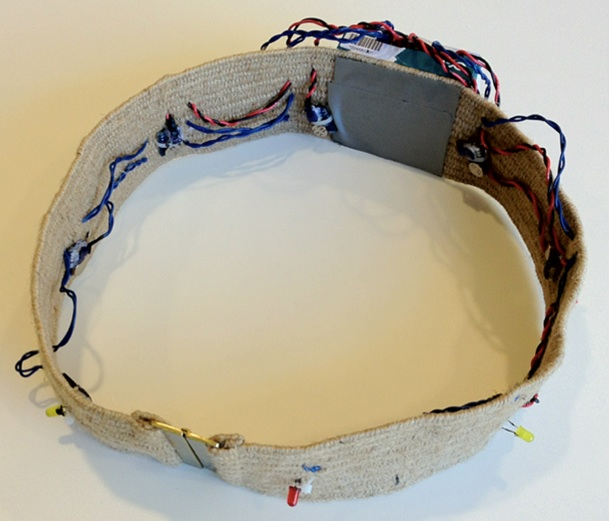
\includegraphics[width=0.35\textwidth]{pics/belt}
\caption{The haptic belt prototype used for guidance}
\label{fig:belt}
\end{figure}

\subsection{Hardware}

8 coin type vibration motors are placed uniformly placed around the belt. Although coin motors provide less strength than cylindrical motors, their size and shape make them ideal for the belt application. The motors have 3V rated voltage, 9000 rpm rotation, 90 mA rated current and a maximum 50db mechanical noise and they are driven by a single ULN2803A chip with Pulse Width Modulation (PWM) at 20 kHz.

For controlling the belt, we chose an Arduino, which is a relatively cheap open source electronics prototyping platform. The communication between the Controller PC and the belt is achieved by a RS-232 serial port. Arduino Uno has a built-in USB-to-serial converter and the electronics are powered by this USB port.

\subsection{Software}

Our system makes use of the Robot Operating System (ROS) software infrastructure for interprocess communication and message passing. Controller PC sends messages to Arduino on belt, which consists of a bit array for each of the 8 motors. A bit in the array indicates if the motor is going to vibrate or not, during the corresponding time slot of 1/16 seconds. Upon receiving the bit arrays command, Arduino starts executing the bits one by one. Since all the motors are actuated in the main controller loop, the vibrations are synchronous.

\section{Vibration Patterns}

We define two main classes of vibration patterns depending on the type of intended human motion: directional and rotational. Directional patterns induce a motion towards a direction. Rotational patterns induce a rotation around self, which is intended to control the orientation of the human. 




\begin{figure}[ht!]
\centering
%
        \subfigure[]{%
        	\label{fig:directional}
            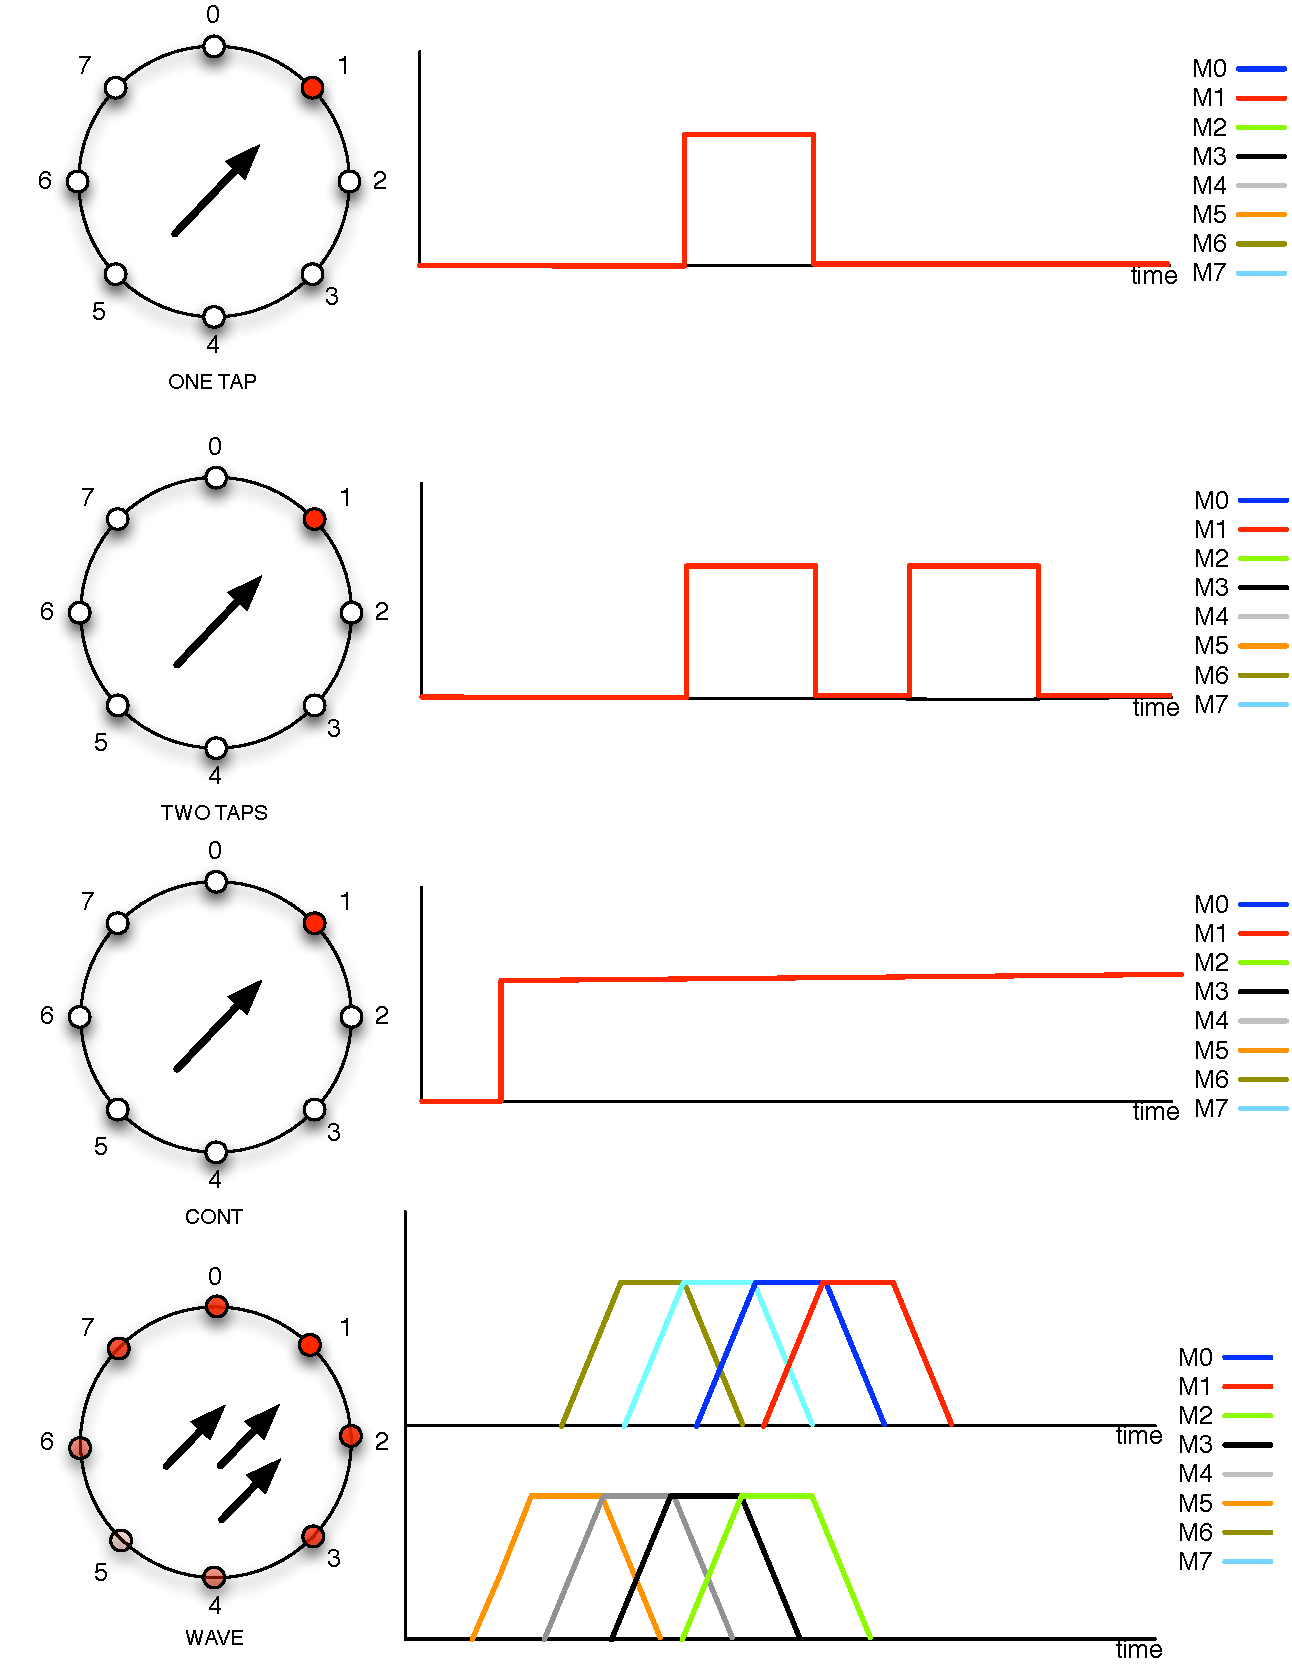
\includegraphics[width=0.46\textwidth]{pics/directional}
        }
        \subfigure[]{%           
            \label{fig:rotational}
           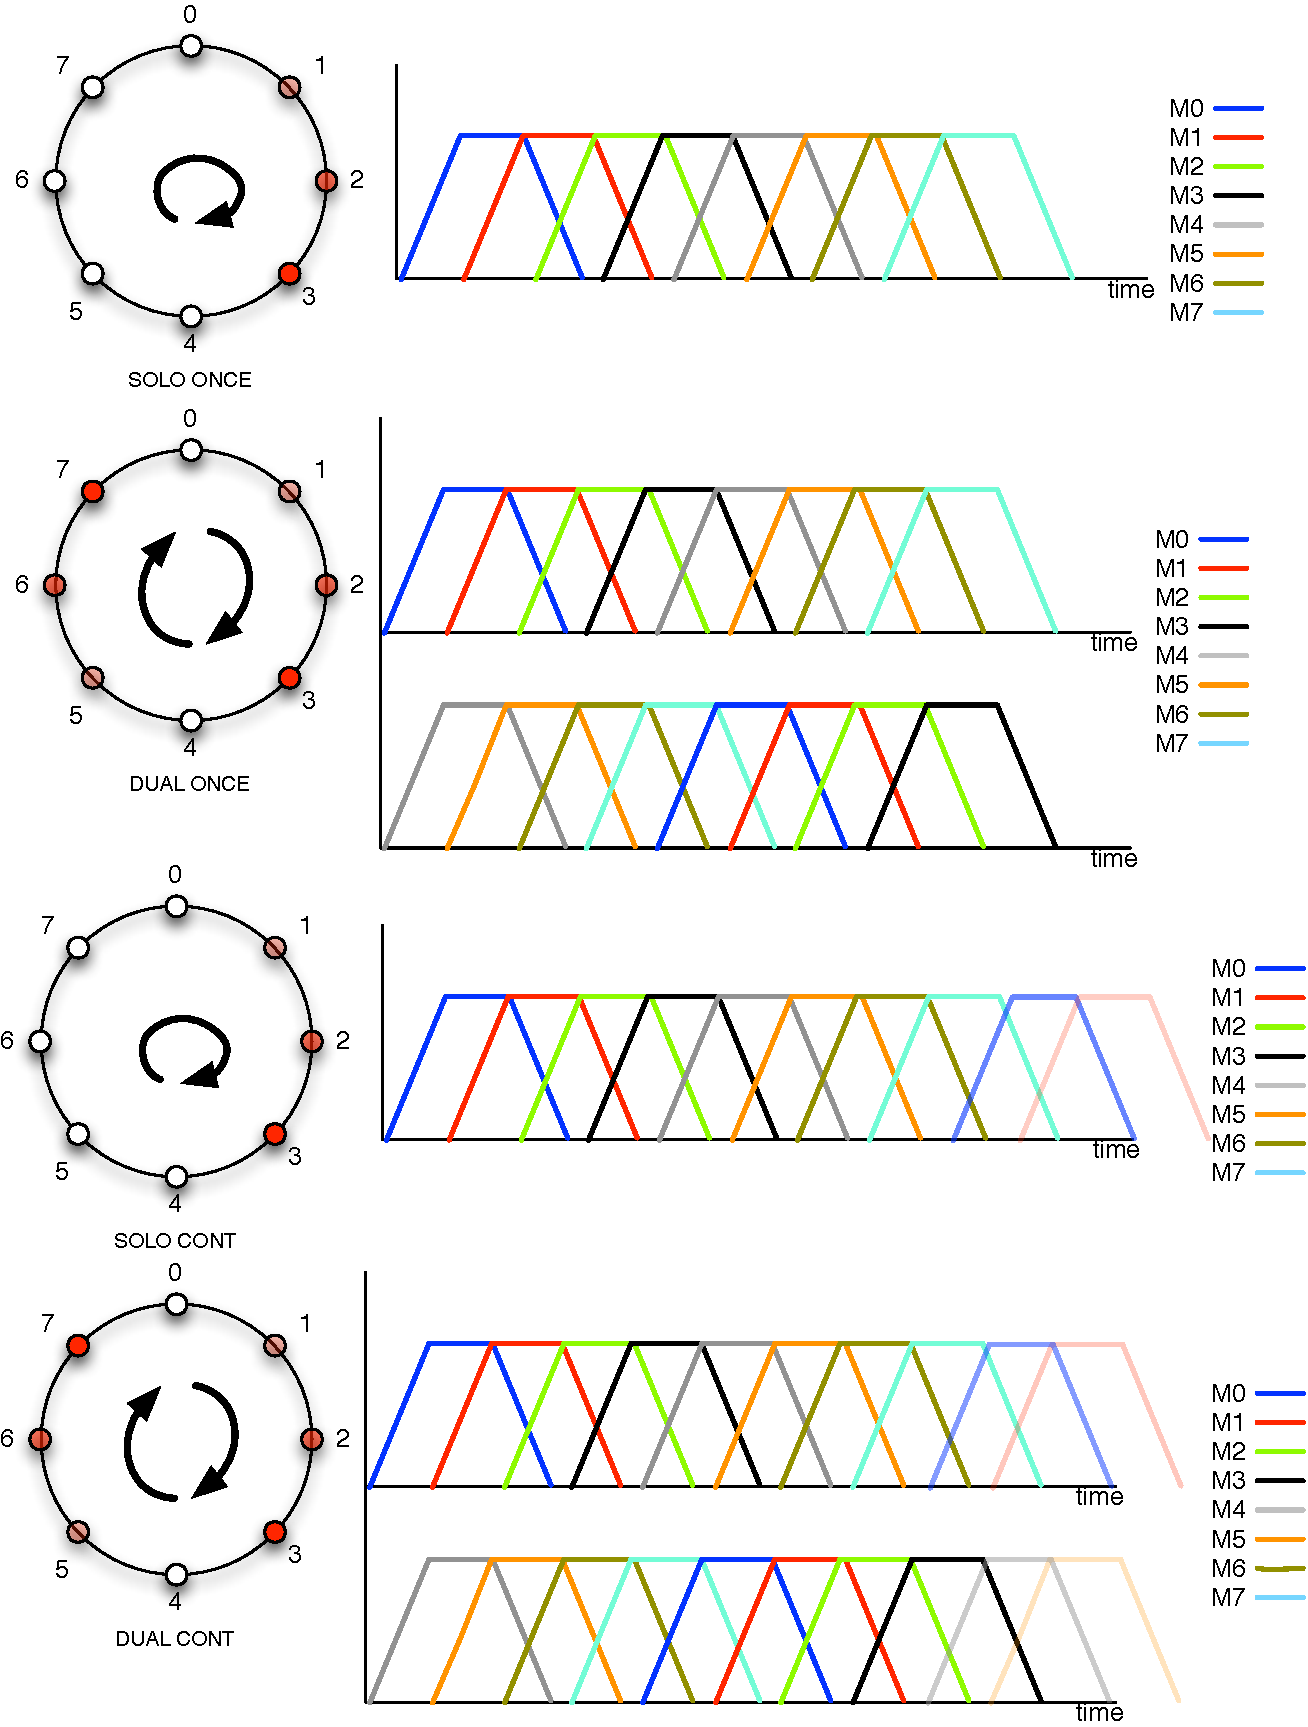
\includegraphics[width=0.46\textwidth]{pics/rotational}
        }        
    \caption{%
	Evaluated vibration patterns. a) Directional b) Rotational
     }%
   \label{fig:directional_rotational}
\end{figure}

\begin{itemize}
\item{\textbf{ONE TAP:} a motor is active for 250ms}
\item{\textbf{TWO TAPS:} a motor is active 250ms, inactive for 250ms and active for 250ms again}
\item{\textbf{CONT:} a motor is active until a new pattern is applied}
\item{\textbf{WAVE:} a feeling that starts from the opposite end of desired direction and ends in desired direction}
\end{itemize}

Figure \ref{fig:directional} illustrates all 4 directional patterns for towards northeast cardinal direction (Vibration Motor 1).

\begin{itemize}
\item{\textbf{SOLO ONCE: } activates all 8 motors consecutively, starting from left motor for clockwise, right  for counter-clockwise.}
\item{\textbf{SOLO CONT: } repeats \textbf{SOLO ONCE} pattern}
\item{\textbf{DUAL ONCE: } circle motion is executed for one full circle with two opposing motors instead of one}
\item{\textbf{DUAL CONT: } repeats \textbf{DUAL ONCE} pattern}
\end{itemize}

Figure \ref{fig:rotational} illustrates all 4 rotational patterns for a clockwise rotation motion. 

\section{Procedure}

The subject first went through a training for 5 minutes where experimenter applied directional and rotational patterns and told the correct direction/rotation. The subject is instructed to walk randomly in a confined area so that the patterns are tested while the human is in motion. The subject was asked to press a button on a Xbox controller whenever he/she decides on the direction/rotation and then tell the direction (coded 1-8) or rotation (left or right). The experiments consisted of 4 studies:

\begin{enumerate}
\item 5 samples from each of the \textbf{ONE TAP, TWO TAPS, WAVE} directional patterns are applied in random order. 
\item 8 samples from \textbf{CONT} directional pattern are applied.
\item 2 samples from each of the 4 rotational patterns are applied.
\item 2 samples from each of the 4 rotational patterns while a random directional motion pattern is applied in between samples.
\end{enumerate}


Upon the completion of the experiment, the experimenter applied all vibration patterns one by one and asked which directional and rotational pattern the he/she would prefer. Then, a post-study survey is conducted.

We hypothesize that subjects will prefer a one-time signal pattern in Experiment 1 to continuous pattern in Experiment 2 because a long lasting vibration may be annoying to the users. Our second hypothesis is that applying intermediate directional patterns will reduce the recognition rate of rotational patterns. This would be tested by comparing Study Experiment 3 and Experiment 4 results.

\section{Measures}

3 metrics were used for evaluation:
\begin{itemize}
\item{\textbf{Recognition error (RE):} Angle difference between applied and perceived direction}
\item{\textbf{Recognition accuracy (RA):} Percentage of correct recognition}
\item{\textbf{Reaction time (RT):}  Time between the start of the pattern to the instant the subject decides on an answer. A timeout occurs if subject can not give an answer in 5 seconds.}
\end{itemize}

The post-survey consisted of 4 usability questions on a 10-point Likert scale. Participants were also asked for their preferred directional and rotational patterns.

\section{Results}
\subsection{Directional Patterns}

\textbf{Recognition error and RT w.r.t. pattern type:} A total of 344 directional pattern samples were sampled in Experiments 1 and 2. Since the directions are discretized, RE from any single test ranges from 0 to $180^{\circ}$ with $45^{\circ}$ increments. Results with respect to pattern type is in Table \ref{tab:dir_results}. 

%%%%%%%%%%%%%
\begin{table}[ht!]
\centering
\begin{tabular}{ r | c | c  | c | c |}
\cline{2-5}
& \footnotesize{ONE TAP} & \footnotesize{TWO TAPS} & \footnotesize{CONT} & \footnotesize{WAVE} \\ \hline
\multicolumn{1}{ |c|}{\scriptsize{Directional Error}}& $12.4^{\circ}$ & $10.6^{\circ}$  & $8.4^{\circ}$ & \multicolumn{1}{r|}{$23.1^{\circ}$} \\ \hline
\multicolumn{1}{ |c|}{\scriptsize{Reaction Time (s)}}& 1.32 & 1.13 & 1.26 & \multicolumn{1}{r|}{1.92}\\ \hline
\end{tabular}
\caption{Average recognition error and reaction times of directional patterns}
\label{tab:dir_results}
\end{table}




With a mean RE of $8.4^{\circ}$, \textbf{CONT} pattern was the most accurate directional pattern, followed by \textbf{TWO TAPS} pattern with $10.6^{\circ}$. Subjects recognized \textbf{TWO TAPS} the fastest by an average of 1.13 seconds. \textbf{WAVE} pattern performed significantly worse than others on both measures.

\textbf{Recognition accuracy w.r.t. applied direction:}
The confusion matrix for RA of the applied directions is given in Table~\ref{fig:vibration_pattern_conf_matrix}.

\begin{figure}[ht!]
\centering
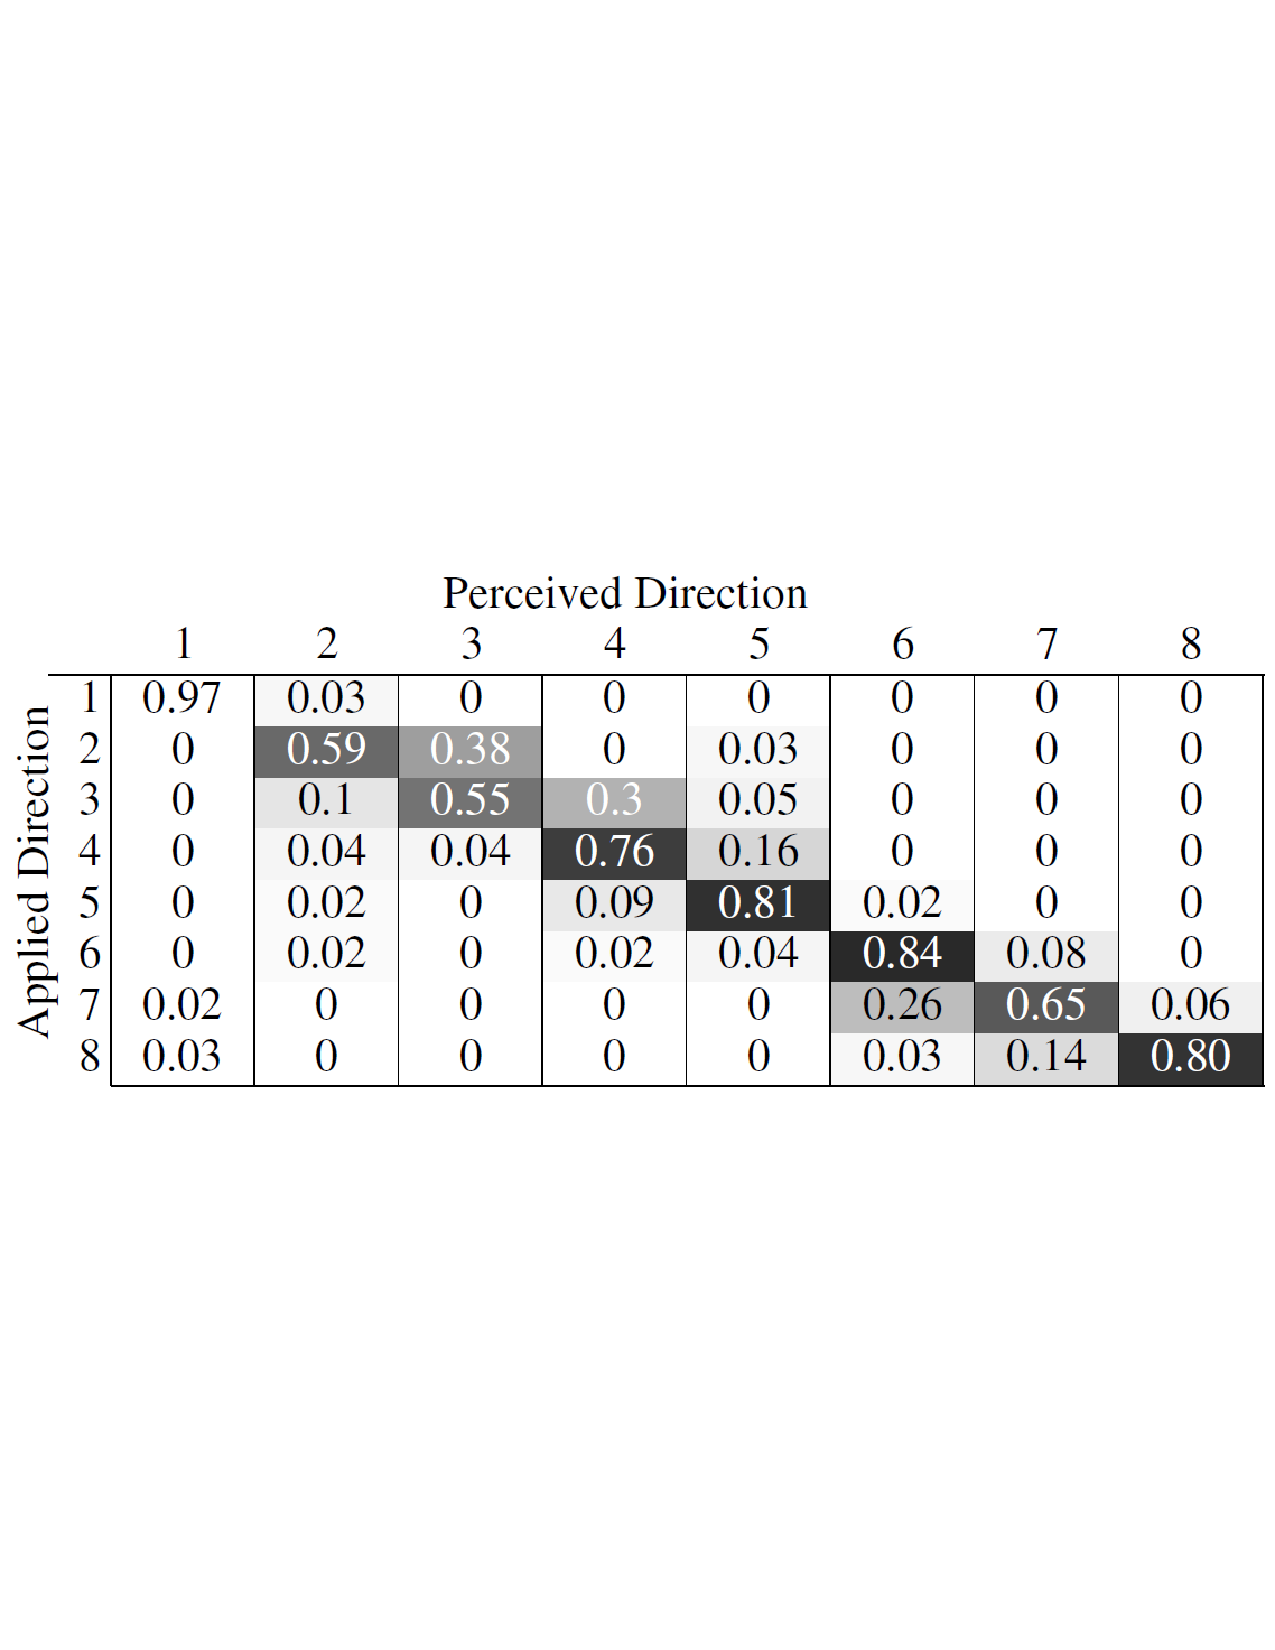
\includegraphics[width=0.85\textwidth]{pics/vibration_pattern_conf_matrix_cropped}
\caption{Confusion matrix of recognition accuracy of directional vibration patterns. Our results show that the recognition accuracy is highly dependent on the applied direction. The subjects recognied the front direction (Direction 1) with the highest accuracy ($\%$97) whereas Direction 3 had the least accuracy ($\%$55)}
\label{fig:vibration_pattern_conf_matrix}
\end{figure}

Our results show that the recognition accuracy is highly dependent on the applied direction. The subjects recognized the front direction with highest RA ($\%$97) whereas Direction 3 (right) had the least RA ($\%$55).

We expected the directional RA to be symmetrical around the belt, meaning that the accuracy of right and left directions should be equally sensitive to haptic feedback. However, there is at least $\%$10 accuracy difference for all 3 such pairs. This could be due to imperfect alignment of motors in the belt prototype.

\subsection{Rotational Patterns}

\begin{table}[ht!]
\centering
\begin{tabular}{ r | c |c |c | c |}
\cline{2-5}
& \footnotesize{SOLO ONCE} & \footnotesize{DUAL ONCE} & \footnotesize{SOLO CONT} & \footnotesize{DUAL CONT} \\ \hline
\multicolumn{1}{ |c|}{\scriptsize{Recog. Accuracy}}& $\%$100 & $\%$92 & $\%$100 & \multicolumn{1}{r|}{$\%$98} \\ \hline
\multicolumn{1}{ |c|}{\scriptsize{Reaction Time (s)}}& 1.32 & 1.84 & 1.16 & \multicolumn{1}{r|}{1.68}\\ \hline
\end{tabular}
\caption{Average recognition accuracy and reaction times of rotational patterns}
\label{tab:rot_results}
\end{table}

A total of 256 rotational pattern samples were tested Experiments 1 and 2. Results are in Figure \ref{tab:rot_results}.

Subjects recognized \textbf{SOLO ONCE} and \textbf{SOLO CONT} patterns with $\% 100$ accuracy, whereas had \textbf{DUAL ONCE} had $\% 92$ RA. \textbf{SOLO CONT} had the least RT by $1.16$ seconds. It is interesting to note that this reaction time is almost identical to the directional pattern with the least RT ($1.13s$).

\subsection{Usability of Tactile Belt}

Subjects thought that it was fairly easy to move while wearing the belt (M=9.2). Most subjects thought that the belt was comfortable (M=8.3) and it fit their waist well (M=8.4). The vibration motors were not found very silent (M=6.8). Actual questions in the post-study survey results are shown in Figure~\ref{fig:survey}. 

\begin{figure}[ht!]
\centering
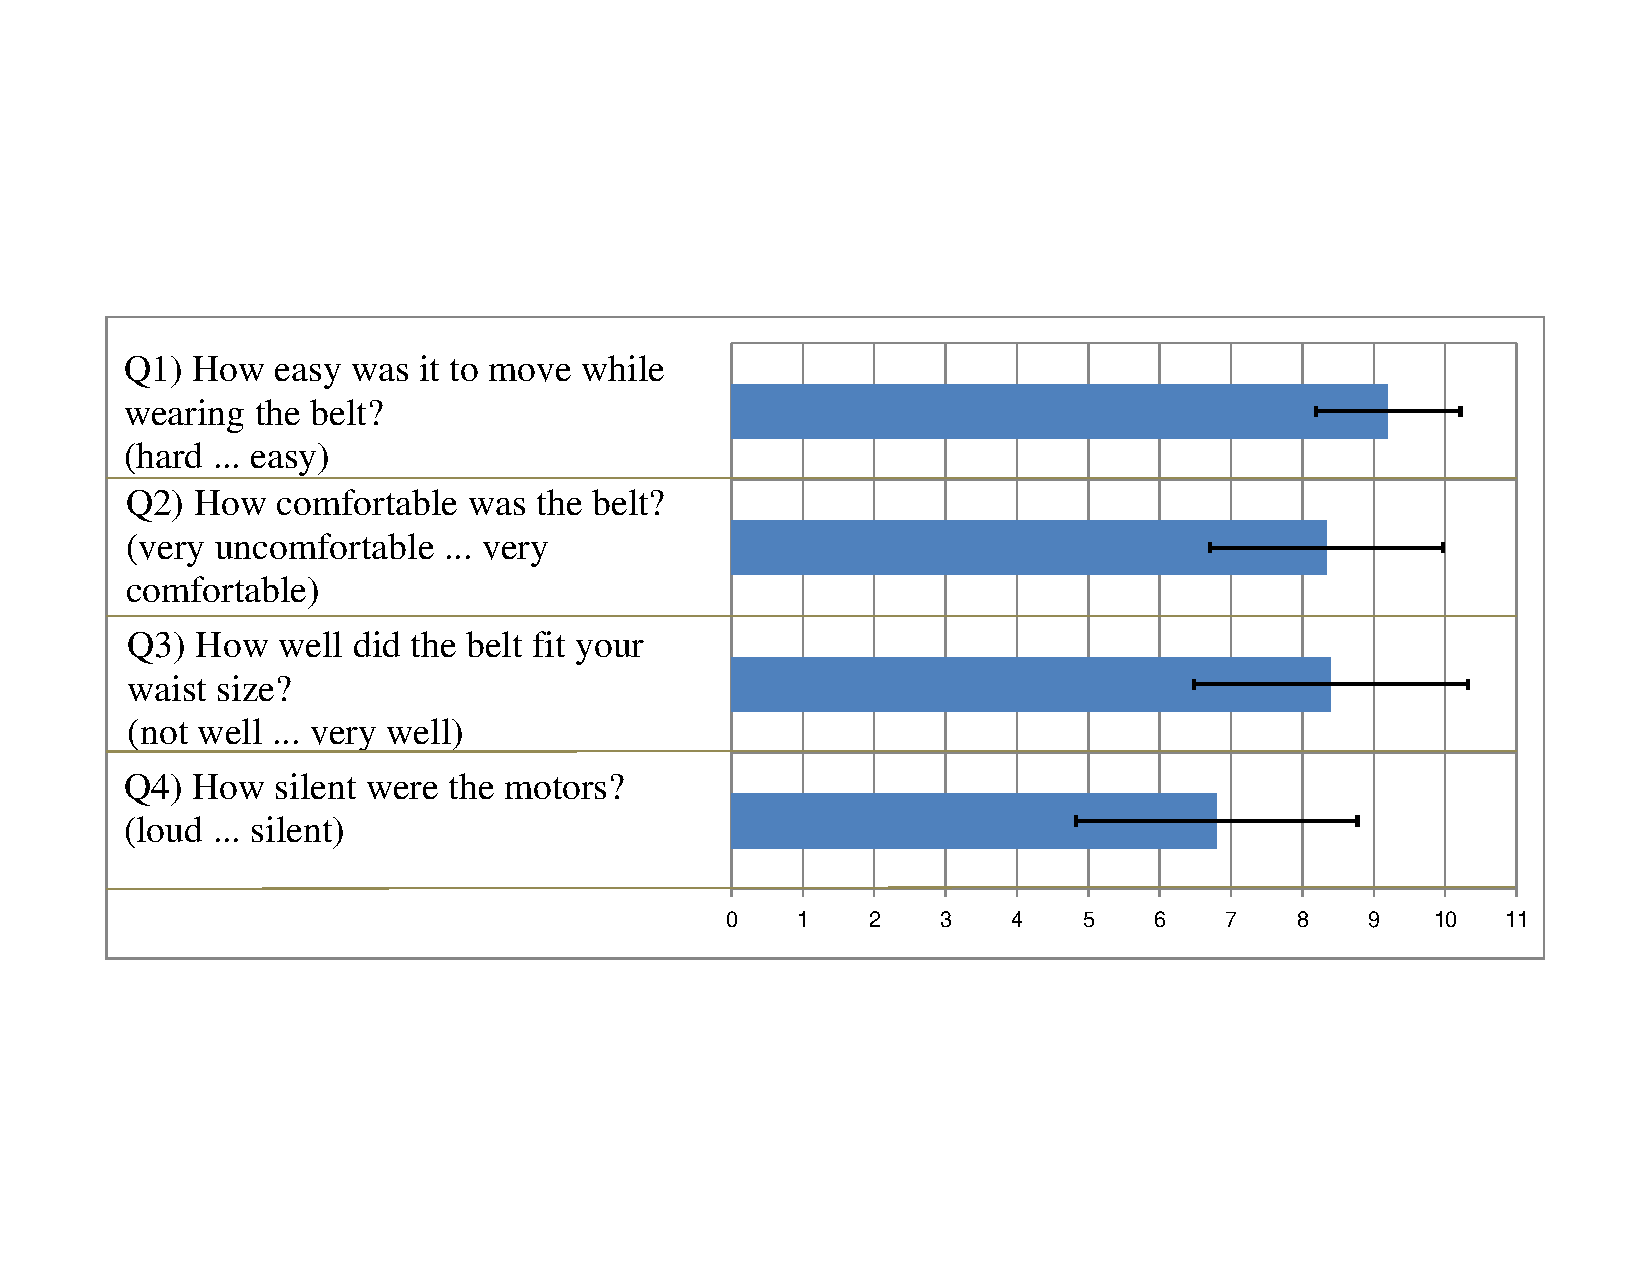
\includegraphics[trim=50 150 50 150,clip, width=1.0\textwidth]{pics/belt_survey}
\caption{Results of post-study survey.}
\label{fig:survey} 
\end{figure}

\subsection{Discussion}

Among directional patterns, \textbf{TWO TAPS} had the least RT and was found the most intuitive by our usability study. When asked which directional pattern they would prefer, 10 out of 15 subjects chose \textbf{TWO TAPS}, 3 subjects chose \textbf{CONT} and 2 subjects selected \textbf{ONE TAP} and no one chose \textbf{WAVE}. Although \textbf{CONT} have less recognition error, most subjects preferred \textbf{TWO TAPS} probably because people didn't feel comfortable when the vibration lasted for a long time. This supports our first hypothesis that continuous patterns would not be found preferable.

7 out of 15 subjects preferred \textbf{SOLO ONCE}, 7 subjects preferred \textbf{SOLO CONT} and 1 subject preferred \textbf{DUAL CONT} in the post-study survey. Our results show that subjects rarely made mistakes in recognizing rotations and using a single motor for rotation patterns is preferable over using two motors. Therefore an application may use either of the \textbf{SOLO} patterns. 

Our second hypothesis did not hold, as we found that application of other pattern between rotational patterns did not deteriorate the recognition rate.